\documentclass{article}

\usepackage{graphicx}
\usepackage{rotating}
\usepackage{amsmath}
\usepackage{amssymb}
\usepackage{fancyhdr}
\usepackage{listings}
\usepackage{xcolor}
\usepackage{color}
\usepackage{amsfonts}
\usepackage{textcomp}
\usepackage{float}
\usepackage[sorting=none]{biblatex}
\usepackage[margin=1in]{geometry}
\usepackage[font={small,it}]{caption}
\usepackage{placeins}
\usepackage{xepersian}

%\DeclareMathOperator*{\btie}{\bowtie}
\addbibresource{bibliography.bib}
\settextfont[Scale=1.2]{B-NAZANIN.TTF}
\setlatintextfont[Scale=1]{Times New Roman}
\renewcommand{\baselinestretch}{1.5}
\pagestyle{fancy}
\fancyhf{}
\rhead{تکلیف دوم درس مبانی یادگیری ماشین (بخش تئوری)}
\lhead{\thepage}
\rfoot{علیرضا ابره فروش}
\lfoot{9816603}
\renewcommand{\headrulewidth}{1pt}
\renewcommand{\footrulewidth}{1pt}
\newcommand{\Lagr}{\mathcal{L}}
%%%%%%%%%%
\lstset
{
    language=[latex]tex,
    basicstyle=\ttfamily,
    commentstyle=\color{black},
    columns=fullflexible,
    keepspaces=true,
    upquote=true,
    showstringspaces=false,
    morestring=[s]\\\%,
    stringstyle=\color{black},
}
%%%%%%%%%%
%beginMatlab
\definecolor{mygreen}{RGB}{28,172,0} % color values Red, Green, Blue
\definecolor{mylilas}{RGB}{170,55,241}
%endMatlab
\begin{document}
%beginMatlab
\lstset{language=Matlab,%
    %basicstyle=\color{red},
    breaklines=true,%
    morekeywords={matlab2tikz},
    keywordstyle=\color{blue},%
    morekeywords=[2]{1}, keywordstyle=[2]{\color{black}},
    identifierstyle=\color{black},%
    stringstyle=\color{mylilas},
    commentstyle=\color{mygreen},%
    showstringspaces=false,%without this there will be a symbol in the places where there is a space
    numbers=left,%
    numberstyle={\tiny \color{black}},% size of the numbers
    numbersep=9pt, % this defines how far the numbers are from the text
    emph=[1]{for,end,break},emphstyle=[1]\color{red}, %some words to emphasise
    %emph=[2]{word1,word2}, emphstyle=[2]{style},    
}
%endMatlab
\begin{titlepage}
\begin{center}

\includegraphics[width=0.4\textwidth]{figures/IUT Logo.png}\\
        
\LARGE
\textbf{دانشگاه صنعتی اصفهان}\\
\textbf{دانشکده مهندسی برق و کامپیوتر}\\
        
\vfill
        
\huge
\textbf{عنوان: تکلیف چهارم درس ریزپردازنده}\\
        
\vfill
        
\LARGE
\textbf{نام و نام خانوادگی: علیرضا ابره فروش}\\
\textbf{شماره دانشجویی: 9816603}\\
\textbf{نیم\,سال تحصیلی: پاییز 1400}\\
\textbf{مدرّس: دکتر عارف کریمی افشار}\\
\end{center}
\end{titlepage}


%\tableofcontents
\newpage


%1
\section{}
\subsection{الف}
\begin{latin}
$
\theta =
\begin{bmatrix}
3 \\
0 \\
-1
\end{bmatrix},
x = 
\begin{bmatrix}
1 \\
x_1 \\
x_2
\end{bmatrix}
$
\end{latin}
مرز تصمیم $\theta ^ t x = 0$ است. پس داریم:
\begin{latin}
$
\theta ^ t x = 0 \\ \Rightarrow 
\left( 3 \right) \times \left( 1 \right) + \left( 0 \right) \times \left( x_1 \right) + \left( -1 \right) \times \left( x_2 \right) = 0 \\ \Rightarrow 
x_2 = 3
$
\end{latin}
مرز تصمیم $x_2 = 3$ است.



\subsection{ب}
\begin{latin}
$
\theta =
\begin{bmatrix}
-2 \\
1 \\
1
\end{bmatrix},
x = 
\begin{bmatrix}
1 \\
x_1 \\
x_2
\end{bmatrix}
$
\end{latin}
مرز تصمیم $\theta ^ t x = 0$ است. پس داریم:
\begin{latin}
$
\theta ^ t x = 0 \\ \Rightarrow 
\left( -2 \right) \times \left( 1 \right) + \left( 1 \right) \times \left( x_1 \right) + \left( 1 \right) \times \left( x_2 \right) = 0 \\ \Rightarrow 
x_2 = -x_1 + 2
$
\end{latin}
مرز تصمیم $x_2 = -x_1 + 2$ است.
\subsection{ج}
\begin{latin}
$
z \ge 0: \quad 0.5 \le \sigma\left( z \right)\le 1 \\
z \le 0: \quad 0 \le \sigma\left( z \right)\le 0.5 \\ \Rightarrow 
\theta^t
\begin{bmatrix}
1 \\
0 \\
0
\end{bmatrix} \le 0 \\
0 \le \theta^t
\begin{bmatrix}
1 \\
0 \\
1
\end{bmatrix} \\
0 \le \theta^t
\begin{bmatrix}
1 \\
1 \\
0
\end{bmatrix} \\
0 \le \theta^t
\begin{bmatrix}
1 \\
1 \\
1
\end{bmatrix} \\ \\ \Rightarrow 
\theta_0+\theta_1\times0+\theta_2\times0 \le 0 \\
\theta_0+\theta_1\times0+\theta_2\times1 \ge 0 \\
\theta_0+\theta_1\times1+\theta_2\times0 \ge 0 \\
\theta_0+\theta_1\times1+\theta_2\times1 \ge 0 \\ \Rightarrow 
\theta =
\begin{bmatrix}
-1 \\
1 \\
1
\end{bmatrix}
$
\end{latin}



%2
\section{}

\begin{latin}
$
z=
\begin{bmatrix}
z_0 \\
z_1 \\
\vdots \\
z_{K-1}
\end{bmatrix},
\sigma \left( z \right) =
\begin{bmatrix}
\frac{e ^ {z_0}}{\sum_{i = 1}^{K-1} e ^ {z_i}} \\
\frac{e ^ {z_1}}{\sum_{i = 1}^{K-1} e ^ {z_i}} \\
\vdots  \\
\frac{e ^ {z_{K-1}}}{\sum_{i = 1}^{K-1} e ^ {z_i}}
\end{bmatrix}
\\
\forall i \in \left\{ 0, \cdots, K - 1 \right\} \\
\sigma (z) _ i = \frac{e^{z_i}}{\sum_{j=0}^{K-1}e^{z_j}} \\
J=\begin{bmatrix}
\frac{\partial \sigma (z) _ 0}{\partial z_0} & \cdots  & \frac{\partial \sigma (z) _ 0}{\partial z_{K-1}} \\
\vdots  & \ddots  & \vdots  \\
\frac{\partial \sigma (z) _ {K - 1}}{\partial z_0} & \cdots  & \frac{\partial \sigma (z) _ {K-1}}{\partial z_{K-1}}
\end{bmatrix} \\
\forall i, j \in \left\{ 0, \cdots, K - 1 \right\}\\ \frac{\partial}{\partial z_j} \ln \left( \sigma (z) _ i \right) = \frac{1}{\sigma (z) _ i}\cdot \frac{\partial \sigma (z) _ i}{\partial z_j} \\ \Rightarrow J_{ij} = 
\frac{\partial \sigma (z) _ i}{\partial z_j} = \sigma (z) _ i \frac{\partial}{\partial z_j} \ln \left( \sigma (z) _ i \right) = \sigma (z) _ i \frac{\partial}{\partial z_j} \left( z_i - \ln \left( \sum_{k=0}^{K-1}e^{z_k} \right) \right) \\ = \sigma (z) _ i \left[ 1\left\{ i=j \right\} - \frac{1}{\sum_{k=0}^{K-1}e^{z_k}} \cdot e^{z_j} \right] = \sigma (z) _ i \left[ 1\left\{ i=j \right\} - \sigma (z) _ j \right] \\ \Rightarrow 
J = 
\begin{bmatrix}
\sigma (z) _ 0\left( 1 - \sigma (z) _0 \right) & -\sigma (z) _ 0 \sigma (z) _ 1 & \cdots & -\sigma (z) _ 0 \sigma (z) _ {K-1} \\
-\sigma (z) _ 1 \sigma (z) _ 0 & \sigma (z) _ 1\left( 1 - \sigma (z) _1 \right) & \cdots & -\sigma (z) _ 1 \sigma (z) _ {K-1} \\
\vdots  & \vdots & \ddots & \vdots \\
-\sigma (z) _ {K-1} \sigma (z) _ 0 & -\sigma (z) _ {K-1} \sigma (z) _ 1 & \cdots & \sigma (z) _ {K-1}\left( 1 - \sigma (z) _{K-1} \right)
\end{bmatrix}
\mathcal{L} \left( y \right) = -\sum_{i=0}^{K-1}y_i \cdot \ln \left( \sigma \left( z \right) _i \right) \\ \\ \Rightarrow
\frac{\partial \mathcal{L}}{\partial z_j} = -\frac{\partial}{\partial z_j} \sum_{i = 0}^{K-1} y_i \cdot \ln\left( \sigma \left( z \right)_i \right) \\=
-\sum_{i = 0}^{K-1} y_i \cdot \frac{\partial}{\partial z_j} \ln\left( \sigma \left( z \right)_i \right) \\= 
-\sum_{i = 0}^{K-1}\frac{y_i}{\sigma \left( z \right)_i} \cdot \frac{\partial \sigma \left( z \right)_i}{\partial z_j} \\
= -\sum_{i = 0}^{K-1}\frac{y_i}{\sigma \left( z \right)_i} \cdot \sigma \left( z \right)_i \cdot \left( 1\left\{ i=j \right\} - \sigma \left( z \right)_j \right) \\= 
-\sum_{i = 0}^{K-1}y_i \cdot \left( 1\left\{ i=j \right\} - \sigma \left( z \right)_j \right) \\
= \sum_{i = 0}^{K-1}y_i \cdot \sigma \left( z \right)_j - \sum_{i = 1}^{K-1} y_i \cdot 1\left\{ i=j \right\} \\
= \sum_{i = 0}^{K-1}y_i \cdot \sigma \left( z \right)_j - y_j \\
= \sigma \left( z \right)_j \cdot \sum_{i = 0}^{K-1}y_i - y_j \\
= \sigma \left( z \right)_j - y_j \\ \\ \Rightarrow
\frac{\partial \mathcal{L}}{\partial z} = \sigma \left( z \right) - y
$
\end{latin}



%3
\section{}
\subsection{الف}
\begin{latin}
$
x^1 =
\begin{bmatrix}
1 \\
4
\end{bmatrix},
x^2 =
\begin{bmatrix}
2 \\
3
\end{bmatrix},
x^3 =
\begin{bmatrix}
4 \\
5
\end{bmatrix},
y^1 = -1, y^2 = -1, y^3 = 1 \\
\mathcal{L}\left( w, b, \alpha \right) = \frac{1}{2} \left\| w \right\|_2^2 - \sum_{i = 1}^{3} \alpha_i\left( y^i\left( x^{i^T}w + b \right) -1 \right) \\=
\frac{1}{2}w^Tw - \sum_{i = 1}^{3} \alpha_iy^ix^{i^T}w - b\left( \sum_{i = 1}^{3} \alpha_i y^i \right) + \sum_{i = 1}^{3} \alpha_i \\ \\ \\ \Rightarrow
\frac{\partial \mathcal{L}}{\partial w} = w - \sum_{i = 1}^{3} \alpha_i y^i x^i = 0 \Rightarrow w^* = \sum_{i = 1}^{3} \alpha_i y^i x^i \\
\frac{\partial \mathcal{L}}{\partial b} = \sum_{i = 1}^{3} \alpha_i y^i = 0 \\ \\ \\ \Rightarrow
w^* = -\alpha_1
\begin{bmatrix}
1 \\
4
\end{bmatrix} -
\alpha_2
\begin{bmatrix}
2 \\
3
\end{bmatrix}+
\alpha_3
\begin{bmatrix}
4 \\
5
\end{bmatrix} \\
-\alpha_1 -\alpha_2 + \alpha_3 = 0 \\ \\ \\ \Rightarrow 
\underset{\alpha_1, \alpha_2, \alpha_3}{\max} \mathcal{L}\left( w, b, \alpha \right) = \underset{\alpha_1, \alpha_2, \alpha_3}{\max} \left[ \sum_{i = 1}^{3} \alpha_i - \frac{1}{2} \sum_{i, j = 1}^{3} y^i y^j \alpha_i \alpha_j x^{i^T} x^j - b\left( \sum_{i = 1}^{3} \alpha_i y^i \right) \right] \\=
\underset{\alpha_1, \alpha_2, \alpha_3}{\max} \left[ \sum_{i = 1}^{3} \alpha_i - \frac{1}{2} \sum_{i, j = 1}^{3} y^i y^j \alpha_i \alpha_j x^{i^T} x^j \right] = \underset{\alpha_1, \alpha_2, \alpha_3}{\max} \left[ -\frac{1}{2} \sum_{i = 1}^{3} \sum_{j = 1}^{3} y^i y^j \alpha_i \alpha_j x^{i^T} x^j + \sum_{i = 1}^{3} \alpha_i \right] \\ \\
x^{1^T}x^1 = 17, x^{1^T}x^2 = 14, x^{1^T}x^3 = 24, x^{2^T}x^2 = 13, x^{2^T}x^3 = 23, x^{3^T}x^3 = 41 \\ \\ \\ \Rightarrow 
\underset{\alpha_1, \alpha_2, \alpha_3}{\max} -\frac{1}{2} \left[ 17\alpha_1^2 + 28\alpha_1\alpha_2 - 48 \alpha_1 \alpha_3 + 13\alpha_2^2 - 46\alpha_2\alpha_3 + 41 \alpha_3^2 \right] + \alpha_1 + \alpha_2 + \alpha_3 \\=
\underset{\alpha_1, \alpha_2, \alpha_3}{\max} -\frac{1}{2}\left[ 17\alpha_1^2 + 28\alpha_1\alpha_2 -48\alpha_1^2 -48\alpha_1\alpha_2 + 13\alpha_2^2 -46\alpha_1\alpha_2 -46\alpha_2^2 + 41\alpha_1^2 +41\alpha_2^2+82\alpha_1\alpha_2\right] + 2\alpha_1+2\alpha_2 \\=
\underset{\alpha_1, \alpha_2, \alpha_3}{\max} -5\alpha_1^2 - 8x^1 =
\begin{bmatrix}
1 \\
4
\end{bmatrix},
x^2 =
\begin{bmatrix}
2 \\
3
\end{bmatrix},
x^3 =
\begin{bmatrix}
4 \\
5
\end{bmatrix},
y^1 = -1, y^2 = -1, y^3 = 1 \\
\mathcal{L}\left( w, b, \alpha \right) = \frac{1}{2} \left\| w \right\|_2^2 - \sum_{i = 1}^{3} \alpha_i\left( y^i\left( x^{i^T}w + b \right) -1 \right) \\=
\frac{1}{2}w^Tw - \sum_{i = 1}^{3} \alpha_iy^ix^{i^T}w - b\left( \sum_{i = 1}^{3} \alpha_i y^i \right) + \sum_{i = 1}^{3} \alpha_i \\ \\ \\ \Rightarrow
\frac{\partial \mathcal{L}}{\partial w} = w - \sum_{i = 1}^{3} \alpha_i y^i x^i = 0 \Rightarrow w^* = \sum_{i = 1}^{3} \alpha_i y^i x^i \\
\frac{\partial \mathcal{L}}{\partial b} = \sum_{i = 1}^{3} \alpha_i y^i = 0 \\ \\ \\ \Rightarrow
w^* = -\alpha_1
\begin{bmatrix}
1 \\
4
\end{bmatrix} -
\alpha_2
\begin{bmatrix}
2 \\
3
\end{bmatrix}+
\alpha_3
\begin{bmatrix}
4 \\
5
\end{bmatrix} \\
-\alpha_1 -\alpha_2 + \alpha_3 = 0 \\ \\ \\ \Rightarrow 
\underset{\alpha_1, \alpha_2, \alpha_3}{\max} \mathcal{L}\left( w, b, \alpha \right) = \underset{\alpha_1, \alpha_2, \alpha_3}{\max} \left[ \sum_{i = 1}^{3} \alpha_i - \frac{1}{2} \sum_{i, j = 1}^{3} y^i y^j \alpha_i \alpha_j x^{i^T} x^j - b\left( \sum_{i = 1}^{3} \alpha_i y^i \right) \right] \\=
\underset{\alpha_1, \alpha_2, \alpha_3}{\max} \left[ \sum_{i = 1}^{3} \alpha_i - \frac{1}{2} \sum_{i, j = 1}^{3} y^i y^j \alpha_i \alpha_j x^{i^T} x^j \right] = \underset{\alpha_1, \alpha_2, \alpha_3}{\max} \left[ -\frac{1}{2} \sum_{i = 1}^{3} \sum_{j = 1}^{3} y^i y^j \alpha_i \alpha_j x^{i^T} x^j + \sum_{i = 1}^{3} \alpha_i \right] \\ \\
x^{1^T}x^1 = 17, x^{1^T}x^2 = 14, x^{1^T}x^3 = 24, x^{2^T}x^2 = 13, x^{2^T}x^3 = 23, x^{3^T}x^3 = 41 \\ \\ \\ \Rightarrow 
\underset{\alpha_1, \alpha_2, \alpha_3}{\max} -\frac{1}{2} \left[ 17\alpha_1^2 + 28\alpha_1\alpha_2 - 48 \alpha_1 \alpha_3 + 13\alpha_2^2 - 46\alpha_2\alpha_3 + 41 \alpha_3^2 \right] + \alpha_1 + \alpha_2 + \alpha_3 \\=
\underset{\alpha_1, \alpha_2, \alpha_3}{\max} -\frac{1}{2}\left[ 17\alpha_1^2 + 28\alpha_1\alpha_2 -48\alpha_1^2 -48\alpha_1\alpha_2 + 13\alpha_2^2 -46\alpha_1\alpha_2 -46\alpha_2^2 + 41\alpha_1^2 +41\alpha_2^2+82\alpha_1\alpha_2\right] + 2\alpha_1+2\alpha_2 \\=
\underset{\alpha_1, \alpha_2, \alpha_3}{\max} -5\alpha_1 + 2\alpha_1+2\alpha_1x^1 =
\begin{bmatrix}
1 \\
4
\end{bmatrix},
x^2 =
\begin{bmatrix}
2 \\
3
\end{bmatrix},
x^3 =
\begin{bmatrix}
4 \\
5
\end{bmatrix},
y^1 = -1, y^2 = -1, y^3 = 1 \\
\mathcal{L}\left( w, b, \alpha \right) = \frac{1}{2} \left\| w \right\|_2^2 - \sum_{i = 1}^{3} \alpha_i\left( y^i\left( x^{i^T}w + b \right) -1 \right) \\=
\frac{1}{2}w^Tw - \sum_{i = 1}^{3} \alpha_iy^ix^{i^T}w - b\left( \sum_{i = 1}^{3} \alpha_i y^i \right) + \sum_{i = 1}^{3} \alpha_i \\ \\ \\ \Rightarrow
\frac{\partial \mathcal{L}}{\partial w} = w - \sum_{i = 1}^{3} \alpha_i y^i x^i = 0 \Rightarrow w^* = \sum_{i = 1}^{3} \alpha_i y^i x^i \\
\frac{\partial \mathcal{L}}{\partial b} = \sum_{i = 1}^{3} \alpha_i y^i = 0 \\ \\ \\ \Rightarrow
w^* = -\alpha_1
\begin{bmatrix}
1 \\
4
\end{bmatrix} -
\alpha_2
\begin{bmatrix}
2 \\
3
\end{bmatrix}+
\alpha_3
\begin{bmatrix}
4 \\
5
\end{bmatrix} \\
-\alpha_1 -\alpha_2 + \alpha_3 = 0 \\ \\ \\ \Rightarrow 
\underset{\alpha_1, \alpha_2, \alpha_3}{\max} \mathcal{L}\left( w, b, \alpha \right) = \underset{\alpha_1, \alpha_2, \alpha_3}{\max} \left[ \sum_{i = 1}^{3} \alpha_i - \frac{1}{2} \sum_{i, j = 1}^{3} y^i y^j \alpha_i \alpha_j x^{i^T} x^j - b\left( \sum_{i = 1}^{3} \alpha_i y^i \right) \right] \\=
\underset{\alpha_1, \alpha_2, \alpha_3}{\max} \left[ \sum_{i = 1}^{3} \alpha_i - \frac{1}{2} \sum_{i, j = 1}^{3} y^i y^j \alpha_i \alpha_j x^{i^T} x^j \right] = \underset{\alpha_1, \alpha_2, \alpha_3}{\max} \left[ -\frac{1}{2} \sum_{i = 1}^{3} \sum_{j = 1}^{3} y^i y^j \alpha_i \alpha_j x^{i^T} x^j + \sum_{i = 1}^{3} \alpha_i \right] \\ \\
x^{1^T}x^1 = 17, x^{1^T}x^2 = 14, x^{1^T}x^3 = 24, x^{2^T}x^2 = 13, x^{2^T}x^3 = 23, x^{3^T}x^3 = 41 \\ \\ \\ \Rightarrow 
\underset{\alpha_1, \alpha_2, \alpha_3}{\max} -\frac{1}{2} \left[ 17\alpha_1^2 + 28\alpha_1\alpha_2 - 48 \alpha_1 \alpha_3 + 13\alpha_2^2 - 46\alpha_2\alpha_3 + 41 \alpha_3^2 \right] + \alpha_1 + \alpha_2 + \alpha_3 \\=
\underset{\alpha_1, \alpha_2, \alpha_3}{\max} -\frac{1}{2}\left[ 17\alpha_1^2 + 28\alpha_1\alpha_2 -48\alpha_1^2 -48\alpha_1\alpha_2 + 13\alpha_2^2 -46\alpha_1\alpha_2 -46\alpha_2^2 + 41\alpha_1^2 +41\alpha_2^2+82\alpha_1\alpha_2\right] + 2\alpha_1+2\alpha_2 \\=
\underset{\alpha_1, \alpha_2, \alpha_3}{\max} \left[ -5\alpha_1^2 - 8\alpha_1\alpha_2 - 4\alpha_2^2 + 2\alpha_1+2\alpha_2 \right] \\ \\ \\
\Rightarrow J = -5\alpha_1^2 - 8\alpha_1\alpha_2 - 4\alpha_2^2 + 2\alpha_1+2\alpha_2 \\
\frac{\partial J}{\alpha_1} = -10\alpha_1 -8\alpha_2 + 2 = 0 \Rightarrow \alpha_1 = -0.8\alpha_2+0.2 \\
\frac{\partial J}{\alpha_2} = -8\alpha_1 -8\alpha_2 + 2 = 0 \Rightarrow 0.64\alpha_2-1.6-8\alpha_2 + 2 = 0 \\ \Rightarrow
\alpha_2 \simeq 0.0543, \alpha_1 \simeq 0.1565, \alpha_3 = 0.2108 \\ \\ \\
w^* \simeq -0.0543
\begin{bmatrix}
1 \\
4
\end{bmatrix} -
0.1565
\begin{bmatrix}
2 \\
3
\end{bmatrix}+
0.2108
\begin{bmatrix}
4 \\
5
\end{bmatrix} =
\begin{bmatrix}
0.4759 \\
0.3673
\end{bmatrix} \\
b^* = -\begin{bmatrix}
1 \\
4
\end{bmatrix}^T\begin{bmatrix}
0.4759 \\
0.3673
\end{bmatrix}-b=1 \Rightarrow b = -2.9451 \\ \\ \\ \\ \\ \Rightarrow 
0.4759x_2+0.3673x_1 - 2.9451 = 0
$
\end{latin}
\subsection{ب}
\begin{figure}[H]
    \centering
    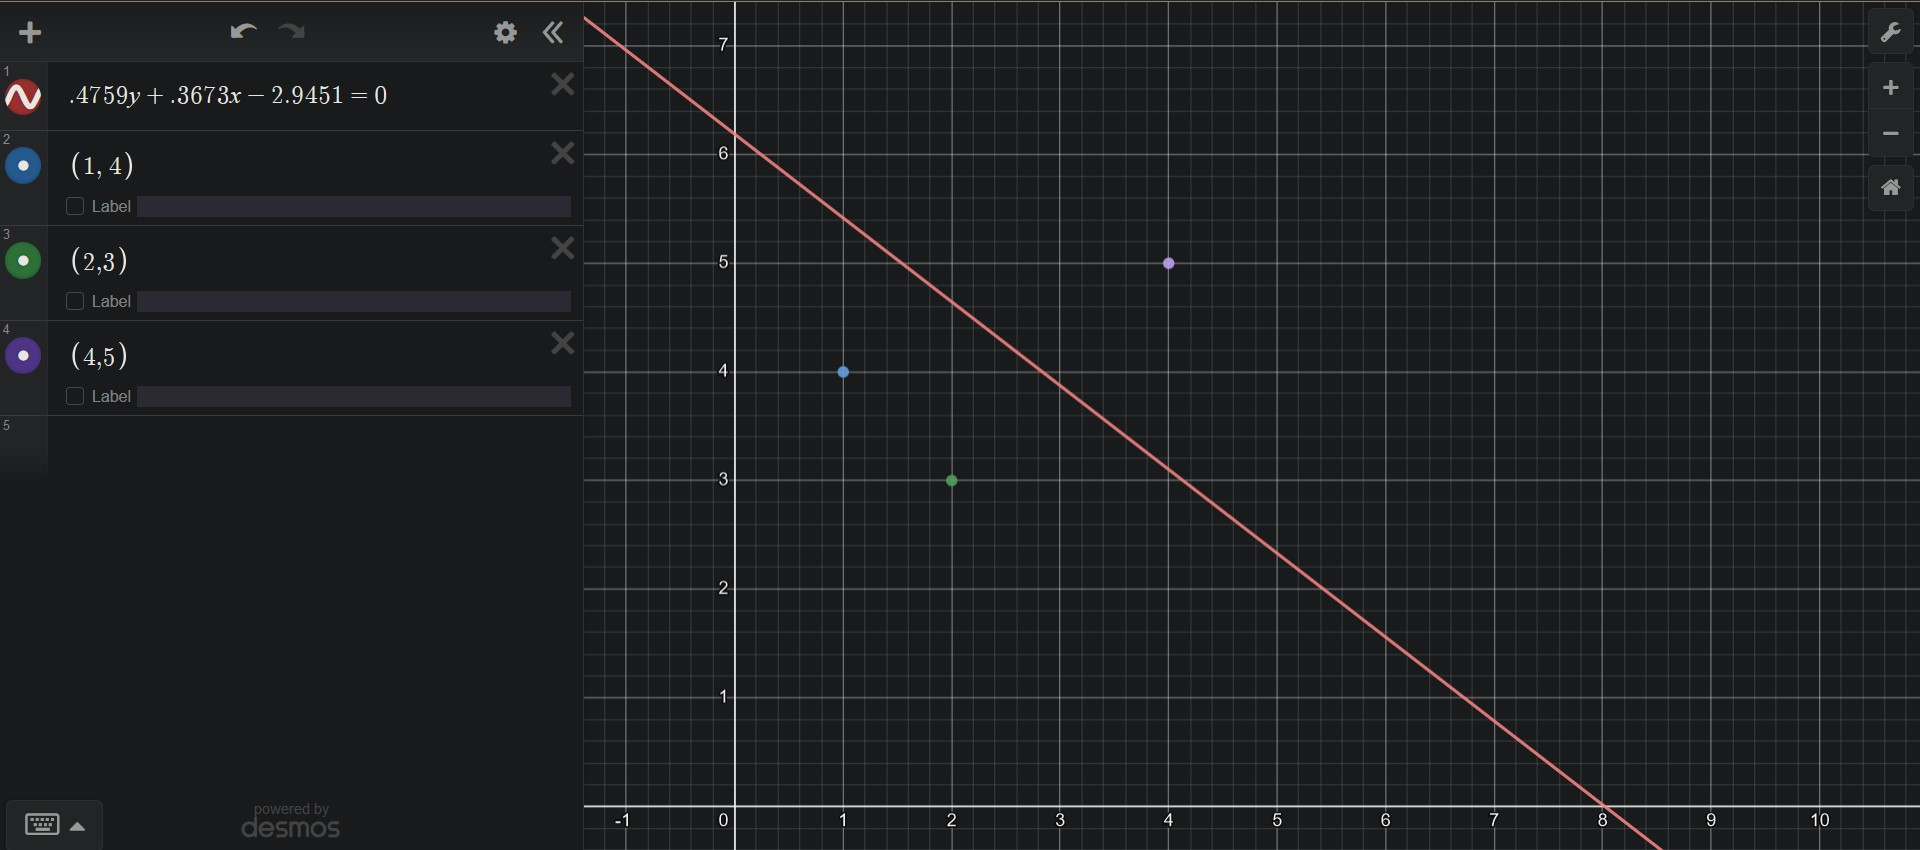
\includegraphics[width=1\textwidth]{figures/1.jpg}
    \caption
	{}
    \label{fig:fig1}
\end{figure}



%4
\section{}
\subsection{الف}
\begin{latin}
$
G\left( D \right) = 1 - \sum_{i=1}^{k} p_i ^ 2 =
1 - \left( p_{c0}^2 + p_{c1}^2 \right) ^ 2 =
1 - \left[ \left( \frac{10}{20} \right) ^ 2 + \left( \frac{10}{20} \right) ^ 2 \right] = \frac{1}{2}
$
\end{latin}

\subsection{ب}
\begin{latin}
$
\forall i \in \left\{ 1, 2, \cdots, 20 \right\}: \quad G_{CustomerID}\left( D_i \right) = 1 - \sum_{j=1}^{k} p_j ^ 2 = 1 - \left( \frac{1}{1} \right)^2 = 0 \\
G_{CustomerID}\left( D \right) = 0
$
\end{latin}

\subsection{ج}
\begin{latin}
$
G_{Gender}\left( D_M \right) = 1 - \left[ \left( \frac{6}{10} \right)^2 + \left( \frac{4}{10} \right)^2 \right] = 0.48 \\
G_{Gender}\left( D_F \right) = 1 - \left[ \left( \frac{4}{10} \right)^2 + \left( \frac{6}{10} \right)^2 \right] = 0.48 \\
\frac{\left| D_M \right|}{D} = \frac{10}{20} = \frac{1}{2} \\
\frac{\left| D_F \right|}{D} = \frac{10}{20} = \frac{1}{2} \\
G_{Gender}\left( D \right) = \frac{1}{2} \times 0.48 + \frac{1}{2} \times 0.48 = 0.48
$
\end{latin}
\subsection{د}
\begin{latin}
$
G_{CarType}\left( D_{Family} \right) = 1 - \left[ \left( \frac{1}{4} \right)^2 + \left( \frac{3}{4} \right)^2 \right] = 0.375 \\
G_{CarType}\left( D_{Sport} \right) = 1 - \left[ \left( \frac{8}{8} \right)^2 \right] = 0 \\
G_{CarType}\left( D_{Luxury} \right) = 1 - \left[ \left( \frac{1}{8} \right)^2 + \left( \frac{7}{8} \right)^2 \right] = 0.21875 \\
\frac{\left| D_{Family} \right|}{D} = \frac{4}{20} = 0.2 \\
\frac{\left| D_{Sport} \right|}{D} = \frac{8}{20} = 0.4 \\
\frac{\left| D_{Luxury} \right|}{D} = \frac{8}{20} = 0.4 \\
G_{CarType}\left( D \right) = 0.2 \times 0.375 + 0.4 \times 0 + 0.4 \times 0.21875 = 0.1625
$
\end{latin}
\subsection{و}
\begin{latin}
$
G_{ShirtSize}\left( D_{Small} \right) = 1 - \left[ \left( \frac{3}{5} \right)^2 + \left( \frac{2}{5} \right)^2 \right] = 0.48 \\
G_{ShirtSize}\left( D_{Medium} \right) = 1 - \left[ \left( \frac{2}{4} \right)^2 + \left( \frac{2}{4} \right)^2 \right] = \frac{24}{49} \\
G_{ShirtSize}\left( D_{Large} \right) = 1 - \left[ \left( \frac{3}{7} \right)^2 + \left( \frac{4}{7} \right)^2 \right] = 0.5 \\
G_{ShirtSize}\left( D_{ExtraLarge} \right) = 1 - \left[ \left( \frac{3}{7} \right)^2 + \left( \frac{4}{7} \right)^2 \right] = 0.5 \\
\frac{\left| D_{Small} \right|}{D} = \frac{5}{20} = 0.25 \\
\frac{\left| D_{Medium} \right|}{D} = \frac{7}{20} = 0.35 \\
\frac{\left| D_{Large} \right|}{D} = \frac{4}{20} = 0.2 \\
\frac{\left| D_{ExtraLarge} \right|}{D} = \frac{4}{20} = 0.2 \\
G_{ShirtSize}\left( D \right) = 0.25 \times 0.48 + 0.35 \times \frac{24}{49} + 0.2 \times 0.5 + 0.2 \times 0.5 \simeq  0.4915
$
\end{latin}
\subsection{ه}
\begin{latin}
$
G_{CarType}\left( D \right) \le G_{Gender}\left( D \right) \le G_{ShirtSize}\left( D \right) 
$
\end{latin}
از آنجایی که ویژگیِ \lr{Car Type} کمترین شاخص \lr{Gini} را دارد پس مناسب‌تر است.
\subsection{ی}
درست است که ویژگیِ \lr{Customer ID} دارای کمترین شاخص \lr{Gini} است. اما چون به ازای هر داده مقدار متمایزی دارد نمی‌توان از آن برای دسته‌بندی استفاده کرد.

%5
\section{}
\subsection{الف}
\begin{latin}
$
E = - \sum_{i = 1}^{k} p_i \log_2 p_i \\ \Rightarrow 
E = - \left( \frac{4}{9} \log_2 \frac{4}{9} + \frac{5}{9} \log_2 \frac{5}{9} \right) \simeq  - \left[ \frac{4}{9} \left( 2-3.17 \right) + \frac{5}{9}\left( 2.32 - 3.17 \right) \right] \simeq 0.99
$
\end{latin}

\subsection{ب}
\begin{latin}
$
E\left( D_T \right) = -\left[ \frac{3}{4} \ log_2 \frac{3}{4} + \frac{1}{4} \ log_2 \frac{1}{4} \right] \simeq 0.815 \\
E\left( D_F \right) = -\left[ \frac{1}{5} \ log_2 \frac{1}{5} + \frac{4}{5} \ log_2 \frac{4}{5} \right] \simeq 0.72 \\
E_{a_1}\left( D \right) = \frac{4}{9} E\left( D_T \right) + \frac{5}{9} E\left( D_F \right) \simeq 0.762  \\
\alpha\left( a_1, D \right) = E\left( D \right) - E_{a_1} \left( D \right) \simeq 0.99 - 0.762 = 0.228 \\ \\
E\left( D_T \right) = -\left[ \frac{2}{5} \ log_2 \frac{2}{5} + \frac{3}{5} \ log_2 \frac{3}{5} \right] \simeq 0.972 \\
E\left( D_F \right) = -\left[ \frac{2}{4} \ log_2 \frac{2}{4} + \frac{2}{4} \ log_2 \frac{2}{4} \right] \simeq 1 \\
E_{a_2}\left( D \right) = \frac{5}{9} E\left( D_T \right) + \frac{4}{9} E\left( D_F \right) \simeq 0.984 \\
\alpha\left( a_2, D \right) = E\left( D \right) - E_{a_2} \left( D \right) \simeq 0.99 - 0.984 = 0.006
$
\end{latin}

\subsection{ج}
\begin{latin}
$
E\left( D_1 \right) = -\left[ \frac{1}{1} \log_2 \frac{1}{1} + \frac{0}{1} \log_2 \frac{0}{1} \right] = 0 \\
E\left( D_3 \right) = -\left[ \frac{0}{1} \log_2 \frac{0}{1} + \frac{1}{1} \log_2 \frac{1}{1} \right] = 0 \\
E\left( D_4 \right) = -\left[ \frac{1}{1} \log_2 \frac{1}{1} + \frac{0}{1} \log_2 \frac{0}{1} \right] = 0 \\
E\left( D_5 \right) = -\left[ \frac{2}{2} \log_2 \frac{2}{2} + \frac{0}{2} \log_2 \frac{0}{2} \right] = 0 \\
E\left( D_6 \right) = -\left[ \frac{1}{1} \log_2 \frac{1}{1} + \frac{0}{1} \log_2 \frac{0}{1} \right] = 0 \\
E\left( D_7 \right) = -\left[ \frac{1}{2} \log_2 \frac{1}{2} + \frac{1}{2} \log_2 \frac{1}{2} \right] = 1 \\
E\left( D_8 \right) = -\left[ \frac{0}{1} \log_2 \frac{0}{1} + \frac{1}{1} \log_2 \frac{1}{1} \right] = 0 \\ \\
E_{a_3}\left( D_1 \right) = \frac{1}{9}E\left( D_1 \right) = 0 \\
E_{a_3}\left( D_3 \right) = \frac{1}{9}E\left( D_3 \right) = 0 \\
E_{a_3}\left( D_4 \right) = \frac{1}{9}E\left( D_4 \right) = 0 \\
E_{a_3}\left( D_5 \right) = \frac{2}{9}E\left( D_5 \right) = 0 \\
E_{a_3}\left( D_6 \right) = \frac{1}{9}E\left( D_6 \right) = 0 \\
E_{a_3}\left( D_7 \right) = \frac{2}{9}E\left( D_7 \right) = \frac{2}{9} \\
E_{a_3}\left( D_8 \right) = \frac{1}{9}E\left( D_8 \right) = 0 \\ \\
\alpha\left( a_3, D_1 \right) \simeq  0.99 - 0 = 0.99 \\
\alpha\left( a_3, D_3 \right) \simeq  0.99 - 0 = 0.99 \\
\alpha\left( a_3, D_4 \right) \simeq  0.99 - 0 = 0.99 \\
\alpha\left( a_3, D_5 \right) \simeq  0.99 - 0 = 0.99 \\
\alpha\left( a_3, D_6 \right) \simeq  0.99 - 0 = 0.99 \\
\alpha\left( a_3, D_7 \right) \simeq  0.99 - \frac{2}{9} \simeq 0.77 \\
\alpha\left( a_3, D_8 \right) \simeq  0.99 - 0 = 0.99 \\ \\ \\
\alpha\left( a_3, D \right) \simeq  0.99 - \frac{2}{9} \simeq 0.77 \\
$
\end{latin}

\subsection{د}
با توجه به اینکه بین $a_1$ و $a_2$ ویژگیِ $a_1$ بیشترین \lr{information gain} را دارد. پس تقسیم‌بندی را بهتر انجام می‌دهد. \\
با توجه به اینکه بین $a_1$ و $a_3$ ویژگیِ $a_3$ بیشترین \lr{information gain} را دارد. پس تقسیم‌بندی را بهتر انجام می‌دهد.

\subsection{و}
\begin{latin}
$
\text{classification error rate}_{a_1} = \frac{2}{9} \\
\text{classification error rate}_{a_2} = \frac{5}{9} \\ \\
\text{classification error rate}_{a_1} \le \text{classification error rate}_{a_2}
$
\end{latin}
با توجه به اینکه ویژگیِ $a_1$ ميزان خطای طبقه‌بندی کمتری دارد تقسیم‌بندی را بهتر انجام می‌دهد.
\subsection{ه}
\begin{latin}
$
G_{a_1}\left( D_T \right) = 1 - \left[ \left( \frac{3}{4} \right) ^ 2 + \left( \frac{1}{4} \right) ^ 2  \right] = \frac{3}{8} = 0.375 \\
G_{a_1}\left( D_F \right) = 1 - \left[ \left( \frac{1}{5} \right) ^ 2 + \left( \frac{4}{5} \right) ^ 2  \right] = \frac{8}{25} = 0.32 \\ \\
G_{a_1}\left( D \right) = \frac{4}{9} \times \frac{3}{8} + \frac{5}{9} \times \frac{8}{25} \simeq 0.35 \\ \\ \\
G_{a_2}\left( D_T \right) = 1 - \left[ \left( \frac{2}{5} \right) ^ 2 + \left( \frac{3}{5} \right) ^ 2  \right] = \frac{12}{25} = 0.48 \\
G_{a_2}\left( D_F \right) = 1 - \left[ \left( \frac{2}{4} \right) ^ 2 + \left( \frac{2}{4} \right) ^ 2  \right] = \frac{1}{2} = 0.5 \\ \\
G_{a_2}\left( D \right) = \frac{5}{9} \times \frac{12}{25} + \frac{4}{9} \times \frac{1}{2} \simeq 0.49
$
\end{latin}
با توجه به اینکه بین $a_1$ و $a_2$ ویژگیِ $a_1$ کمترین شاخص \lr{Gini} را دارد. پس تقسیم‌بندی را بهتر انجام می‌دهد.

%6
\section{}
به طور شهودی با هر بخش‌بندی، داده‌ها همگن‌تر می‌شوند. در نتیجه آنتروپی افزایش نمی‌یابد. در ادامه به اثبات این قضیه می‌پردازیم.
\begin{latin}
$
E \left( D \right) = - \sum_{i = 1}^{k} p_i \log_2 p_i \\ \Rightarrow 
E_{x_i} \left( y \right) = - \sum_{j = 1}^{k} p\left( y_j | x_i \right) \log_2 p\left( y_j | x_i \right) \\
E_x \left( y \right) = - \sum_{i = 1}^{n_x} p\left( x_i \right) E_{x_i}\left( y \right) = - \sum_{i = 1}^{n_x} \sum_{j = 1}^{k} p\left( x_i \right)p\left( y_j | x_i \right) \log_2 p\left( y_j | x_i \right) = - \sum_{i = 1}^{n_x} \sum_{j = 1}^{k} p\left( y_j, x_i \right) \log_2 p\left( y_j | x_i \right) \\ \Rightarrow 
E_x \left( y \right) - E \left( y \right) = - \sum_{i = 1}^{n_x} \sum_{j = 1}^{k} p\left( y_j, x_i \right) \log_2 p\left( y_j | x_i \right) - \left[ - \sum_{i = 1}^{n_x} \sum_{j = 1}^{k} p\left( y_j, x_i \right) \log_2 p\left( y_j \right) \right] \\= 
\sum_{i = 1}^{n_x} \sum_{j = 1}^{k} p\left( y_j, x_i \right) \log_2 \frac{p\left( y_j \right)}{p\left( y_j | x_i \right)} = \sum_{i = 1}^{n_x} \sum_{j = 1}^{k} p\left( y_j, x_i \right) \log_2 \frac{p\left( y_j \right)}{\frac{p\left( y_j, x_i \right)}{p\left( x_i \right)}} = \sum_{i = 1}^{n_x} \sum_{j = 1}^{k} p\left( y_j, x_i \right) \log_2 \frac{p\left( y_j \right)p\left( x_i \right)}{p\left( y_j, x_i \right)} \\ \\
\le \log_2 \left[ \sum_{i = 1}^{n_x} \sum_{j = 1}^{k} p\left( y_j, x_i \right) \log_2 \frac{p\left( y_j \right)p\left( x_i \right)}{p\left( y_j, x_i \right)} \right] = \log_2 \left[ \sum_{i = 1}^{n_x} p\left( x_i \right) \sum_{j = 1}^{k} p\left( y_j \right) \right] = \log_2 1 = 0 \\ \\ \\ \Rightarrow
E_x \left( y \right) \le E \left( y \right)
$
\end{latin}

%7
\section{}
\begin{latin}
$
\underset{\beta_0, \beta}{\min} \sum_{i = 1}^{N}\left[ 1-y_if\left( x_i \right) \right]_+ + \frac{\lambda}{2}\left\| \beta \right\| ^ 2 \overset{\lambda = \frac{1}{C}}{=}
\underset{\beta_0, \beta}{\min} \sum_{i = 1}^{N}\left[ 1-y_if\left( x_i \right) \right]_+ + \frac{1}{2C}\left\| \beta \right\| ^ 2 \\ 
\underset{\times C}{\Rightarrow}
\underset{\beta_0, \beta}{\min} \frac{1}{2}\left\| \beta \right\| ^ 2 +  C \sum_{i = 1}^{N}\left[ 1-y_if\left( x_i \right) \right]_+ \overset{1-y_if\left( x_i \right) \le \zeta_i}{=}
\underset{\beta_0, \beta}{\min} \frac{1}{2}\left\| \beta \right\| ^ 2 +  C \sum_{i = 1}^{N}\left[ \zeta_i \right]_+ \\ \overset{\zeta_i \ge 0}{=}
\underset{\beta_0, \beta}{\min} \frac{1}{2}\left\| \beta \right\| ^ 2 +  C \sum_{i = 1}^{N} \zeta_i 
$
\end{latin}



%%%%%%%%%%%%%%%%%%%%%%%%%%%%%%%%%%%
%%%%%%%%%%%%%%%%%%%%%%%%%%%%%%%%%%%
%%%%%%%%%%%%%%%%%%%%%%%%%%%%%%%%%%%






\section*{منابع}
\renewcommand{\section}[2]{}%
\begin{thebibliography}{99} % assumes less than 100 references
%چنانچه مرجع فارسی نیز داشته باشید باید دستور فوق را فعال کنید و مراجع فارسی خود را بعد از این دستور وارد کنید


\begin{LTRitems}

\resetlatinfont

\bibitem{b1}
\end{LTRitems}

\end{thebibliography}


\end{document}
